\chapter{Multivariate data}
\label{outline}

\section{The nature of multivariate data}
\label{overview}

We will attempt to clarify what we mean by multivariate analysis in the next section, however it is worth noting that much of the data examined is observational rather than collected from designed experiments.   It is also apparent that much of the methodology has been developed outside the statistical literature.   Our primary interest will be in examining continuous data, the only exception being categorical variables indicating group membership.   This may be slightly limiting, but we will also tend to rely on at least asymptotic approximations to (multivariate) normality, although these are not always necessary for some techniques.   The multivariate normal distribution is a fascinating subject in its own right, and experience (supplemented with some brutal transformations) indicates it is a reasonable basis for much work.   Nevertheless, there is considerable interest in robust methods at the moment and we refer to some of theseapproaches where possible.

\section{The role of multivariate investigations}
\label{role}

If we assume that linear and generalised linear models (and their descendants) are the mainstay of statistical practice, there is a sense in which most statistical analysis is multivariate.   However, \emph{multivariate analysis} has come to define a canon of methods which could be characterised by their use of the dependence structure between a large number of variables.   This canon has not yet been firmly established; we attempt one definition of it here but omit some methods others would include and include some methods others would omit.   We would suggest that multivariate analysis has either the units as a primary focus, or involves an assessment primarily of the variables.   When considering the units, we usually refer to techniques for classification; supervised classfication if we already understand the grouping and unsupervised classification where we have no \textit{a priori} knowledge of any groupings within our observed units.   The multivariate methodology at the core of supervised classification is discriminant analysis, although the machine learning community has developed many other approaches to the same task.  We will consider these techniques in the light of hypothesis tests (Hotelling's T$^{2}$ test and Multivariate Analysis of Variance) which might help us determine whether groupings within our data really are distinct.   Unsupervised classification has traditionally been associated with cluster analysis, a wide range of algorithms which attempt to find structure in data.   It is perhaps cluster analysis that is the most often contested component of our multivariate canon - some authorities prefer approaches based less on automated algorithms and rather more on statistical models and would argue for approaches such as mixture models and perhaps latent class analysis.   Given the reliance of cluster analysis on distance measures, we will also consider scaling techniques as a method of visualising distnace.   

In considering the relationship between variables, we will spend some time exploring principal components, the most misused of all multivariate techniques which we consider primarily as a projection technique.   Some coverage will also be given to canonical correlation, an attempt to understand the relationship between two sets of variables.   Finallly, we will consider factor analysis, a much contested technique in statistical circles but a much used one in applied settings.

In order to make some sense of these techniques, we will present a brief overview of linear algebra as it pertains to the techniques we wish to explore, and will present some properties of the multivariate normal distribution.



%\chapter{Presenting Multivariate Data}

\section{Summarising multivariate data (presenting data as a matrix, mean vectors, covariance matrices}
\label{summary}


A number of datasets will be used thoughout the course, where these are not available within R itself they will be posted in the student portal.  For now, consider the \emph{USArrests} data.  This was published by McNeil, D. R. (1977) ``Interactive Data Analysis'', Wiley, and gives Arrest rates in 1973 (derived from World Almanac and Book of facts 1975.  and Urban population rates derived from Statistical Abstracts of the United States 1975.  We therefore consider data on  ``Murder'' (arrests per 100,000), Assault (arrests per 100,000), Rape (arrests per 100,000) and the percentage of the population living in urban areas in each state. 

\subsection{Data display}

A matrix is a convenient way of arranging such data.

\singlespacing
\begin{displaymath}
\begin{array}{lcccc}
....................State & Murder & Assault & Rape &  UrbanPop(\%)\\
\end{array}
\end{displaymath}
\begin{displaymath}
\left[ \begin{array}{lrrrr}
Alabama       &   13.2  &   236  &     21.2 &  58\\
Alaska         &  10.0   &  263  &    44.5 & 48\\
Arizona        &   8.1  &   294   &    31.0 &  80\\
Arkansas     &     8.8 &    190  &     19.5 &  50\\
California    &    9.0  &   276  &     40.6 & 91\\
Colorado       &   7.9  &   204  &     38.7 & 78\\
Connecticut   &    3.3  &   110    &   11.1 & 77\\
Delaware      &    5.9  &   238  &     15.8 & 72\\
Florida       &   15.4  &   335   &    31.9 & 70\\
Georgia     &     17.4  &   211    &   25.8 & 60\\
Hawaii       &     5.3  &    46    &   20.2 & 83\\
$\ldots$ & $\ldots$ & $\ldots$ & $\ldots$ \\
\end{array}
\right]
\end{displaymath}
\onehalfspacing

Note in total that there are 50 states, (this display had been cut off after the 11th row, Hawaii), and that there are four variables.   Have a look at the USArrests data itself, and the associated helpfile:

\begin{verbatim}
> ?USArrests
> summary(USArrests)
> USArrests
\end{verbatim}


\section{Graphical and dynamic graphical methods}
\label{eda}



\subsection{Chernoff's Faces}

One of the more charismatic ways of presenting multivariate data was proposed by Chernoff, H. (1973) ``The use of faces to represent statistical association'', JASA, 68, pp 361-368. (see www.wiwi.uni-bielefeld.de/~wolf/ for the R code to create these).   If you have loaded the mvmmisc.R file, you can get these by typing:

\begin{verbatim}
> faces(USArrests}
\end{verbatim}


\begin{figure}
\begin{center}
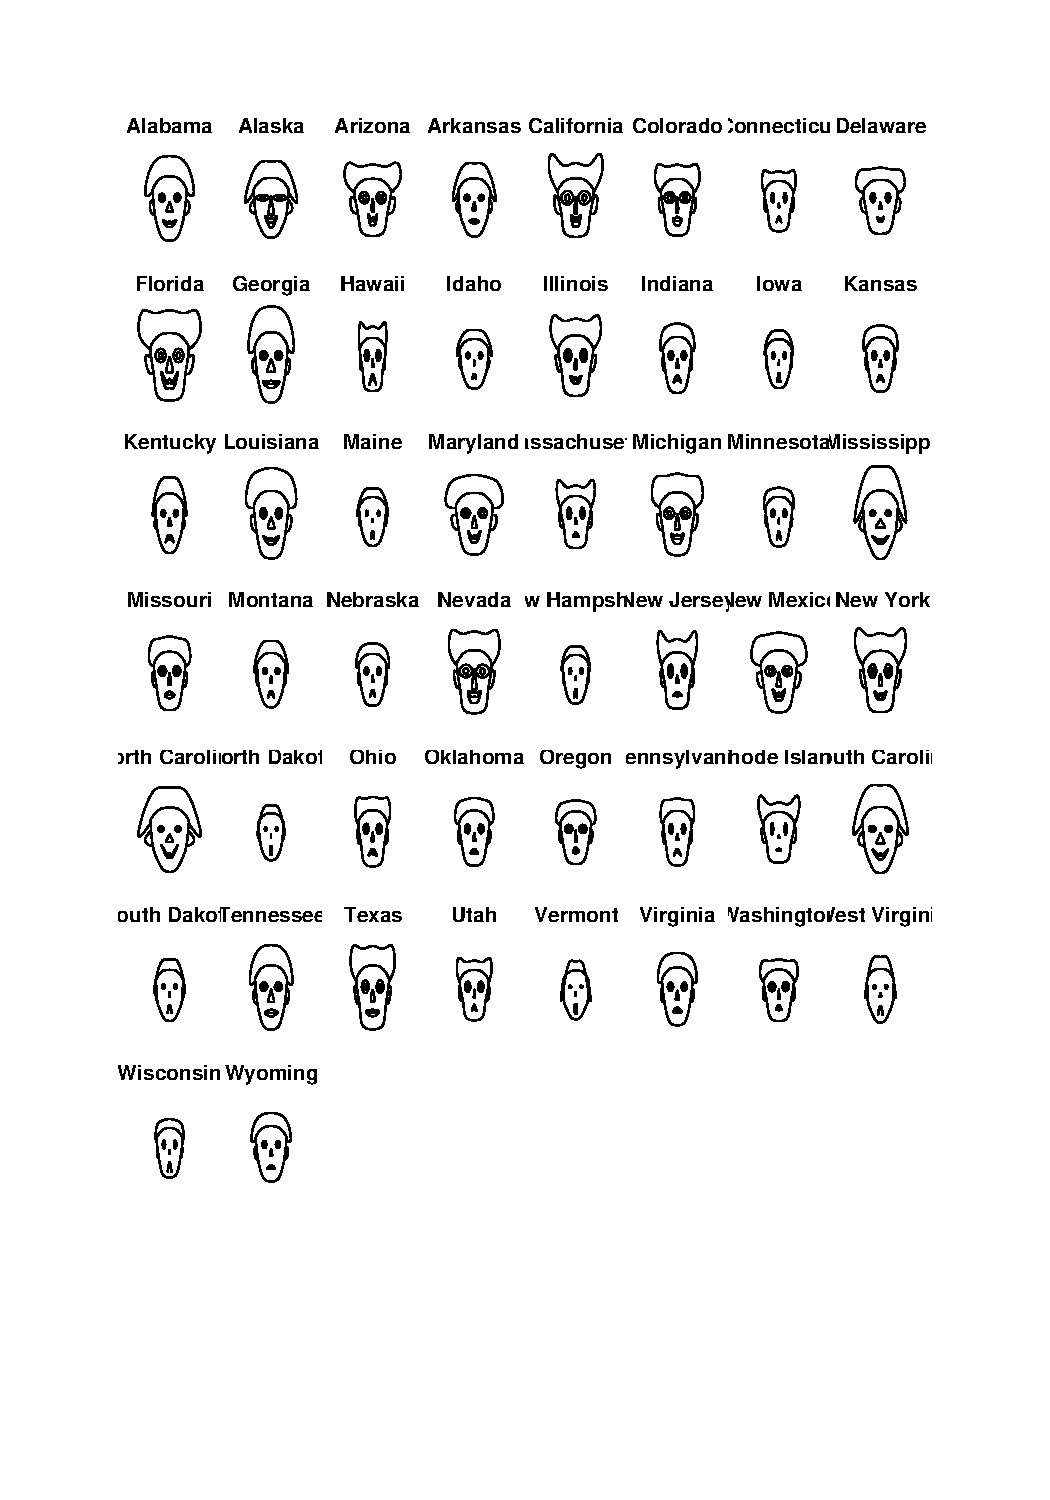
\includegraphics[width = 0.6\textwidth]{images/faces}
\caption{US Arrest data presented as Chernoff's faces}
\end{center}
\end{figure}

However, there are more useful ways of investigating multivariate data.   Slightly less wild, there are star plots, which depict the data as beams.   There are as many beams as there are variables, and the length of the beam reflects the value of the variable.

\singlespacing
\begin{verbatim}
> stars(USArrests)
\end{verbatim}
\onehalfspacing


\subsection{Scatterplots, pairwise scatterplots (draftsman plots)}

Scatterplots should already be familiar as a means of exploring the relationship between two variables.

\singlespacing
\begin{verbatim}
> attach(USArrests)
> plot(Murder, Assault)
> par(las = 1) ## Horizontal axis units on y axis
> plot(Murder, Assault, main = "Scatter plot", pch = 16) 
> detach(USArrests)
\end{verbatim}
\onehalfspacing

\begin{figure}
\begin{center}
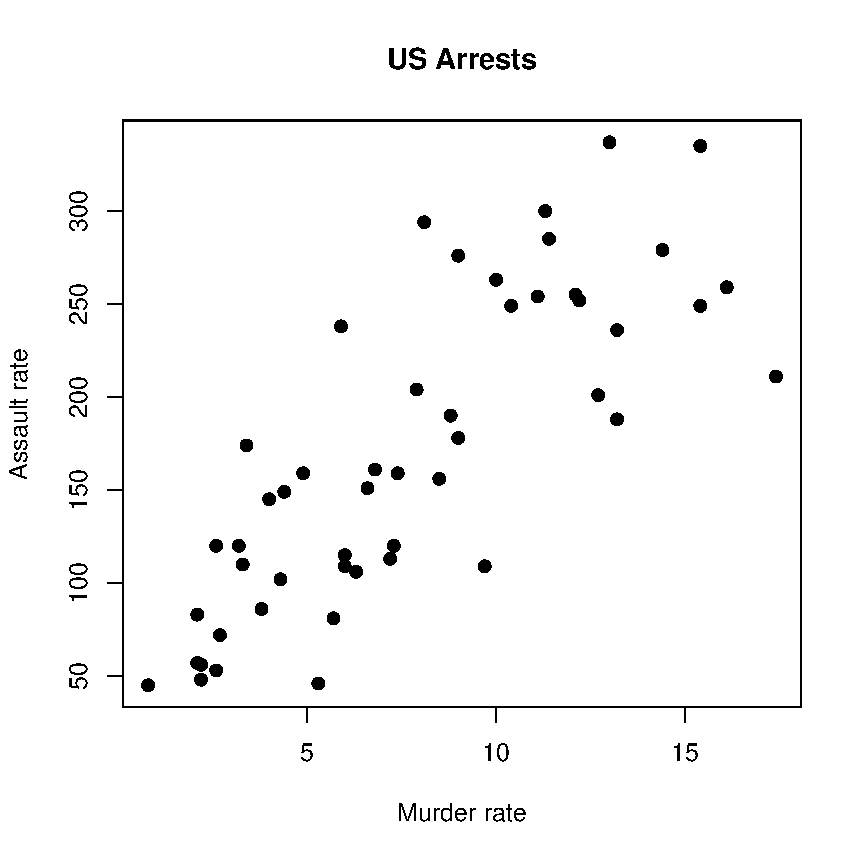
\includegraphics[width = 0.4\textwidth]{images/scatter}
\caption{Scatter plot of Murder rate against Assault rate for US States in 1973}
\end{center}
\end{figure}


However, we have more than two variables of interest.   A set of pairwise scatterplots (sometimes called a draftsman plot) may be of use:

\singlespacing
\begin{verbatim}
> pairs(USArrests, pch = 16)
\end{verbatim}
\onehalfspacing

\begin{figure}
\begin{center}
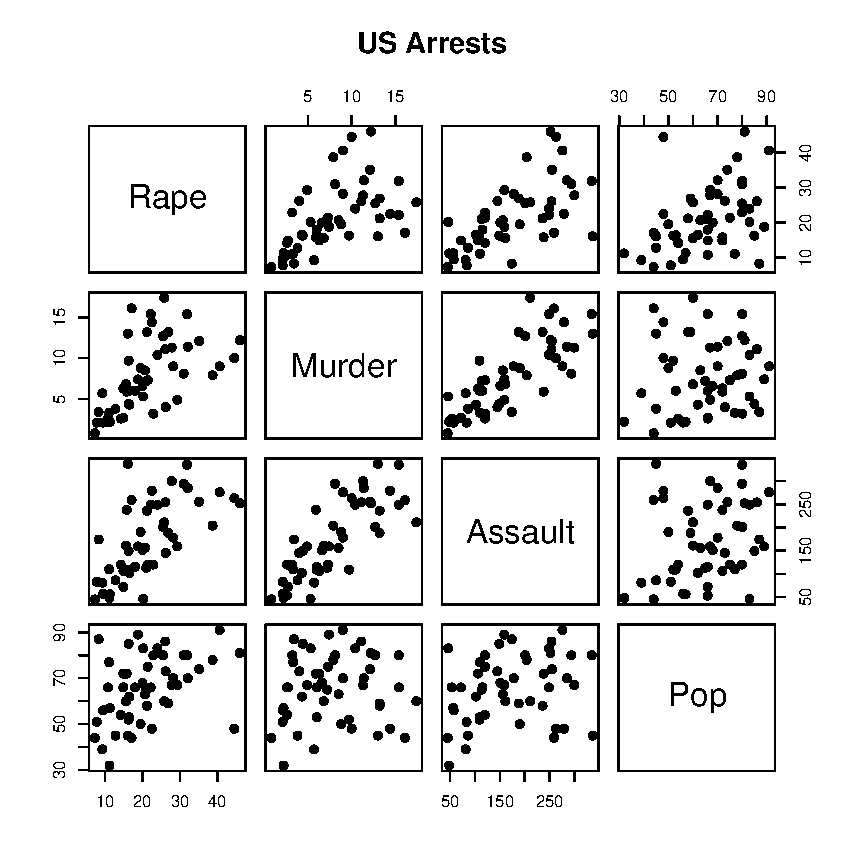
\includegraphics[width = 0.5\textwidth]{images/pairs}
\caption{Pairwise scatter plots for three US arrest rates and percent of population living in Urban areas}
\end{center}
\end{figure}

There other useful functions available.   For example what does \texttt{splom} do?    (Look up \texttt{>?splom}).

\singlespacing
\begin{verbatim}
> library(lattice)
> splom(~USArrests)
\end{verbatim}
\onehalfspacing


\subsection{Optional: 3d scatterplots}

This bit is optional: feel free to have a go if you want to find out about installing R libraries.   

There are facilities in R for making 3d effect scatterplots: you need to download and install an additional library, and when you load the library you need to tell R where to find it.   It is just possible to envisage the three dimensions on the printed page.

\singlespacing
\begin{verbatim}
> install.packages("scatterplot3d", lib = "u:/STAT3401/mvm")
> library(scatterplot3d, lib.loc = "u:/STAT3401/mvm/")
> data(trees)
>  s3d <- scatterplot3d(USArrests[,-3], type="h", highlight.3d=TRUE,
      angle=55, scale.y=0.7, pch=16, main = "USArrests")
\end{verbatim}
\onehalfspacing

\begin{figure}
\begin{center}
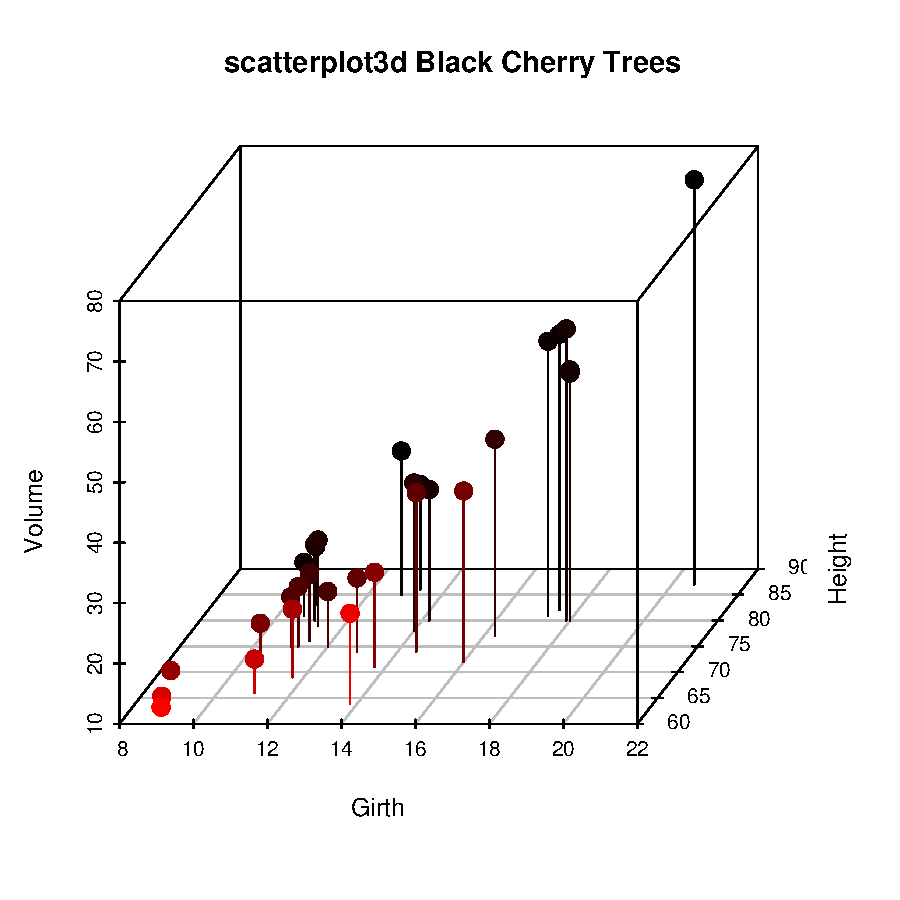
\includegraphics[width = 0.4\textwidth]{images/scat3d}
\caption{3d scatterplot of US arrests}
\end{center}
\end{figure}


\subsection{Other methods}

Other useful methods will be considered in the lab-session, such as glyphs and arrows.   For example there is a rather simple glyph plot available here:

\begin{verbatim}
glyphs(Assault, Murder, Rape, UrbanPop)
\end{verbatim}

The idea of the glyph is that two of the variables are represented as the x and y co-ordinates (as usual), but a futher variable can be represented by the angle of the arrow, and a fourth variable as the length of the arrow.

Interactive graphics offer these facilities, and many more.   There are programs such as GGobi (\texttt{www.ggobi.org}) which allow extensive multivariate investigation such as linked / brushed plots and ``grand tours''.   

\subsection{Profiles}

Just as much ingenuity was extended before modern colour systems.   Another approach is Andrews Curves, described as a function between $-\pi < t < \pi$


\begin{displaymath}
f_{x}(t) = x_{1}/\sqrt 2 + x_{2} \sin 2 + x_{3} \cos t + x_{4} \sin 2t + x_{5} \cos 2t + \ldots
\end{displaymath}

\begin{figure}
\begin{center}
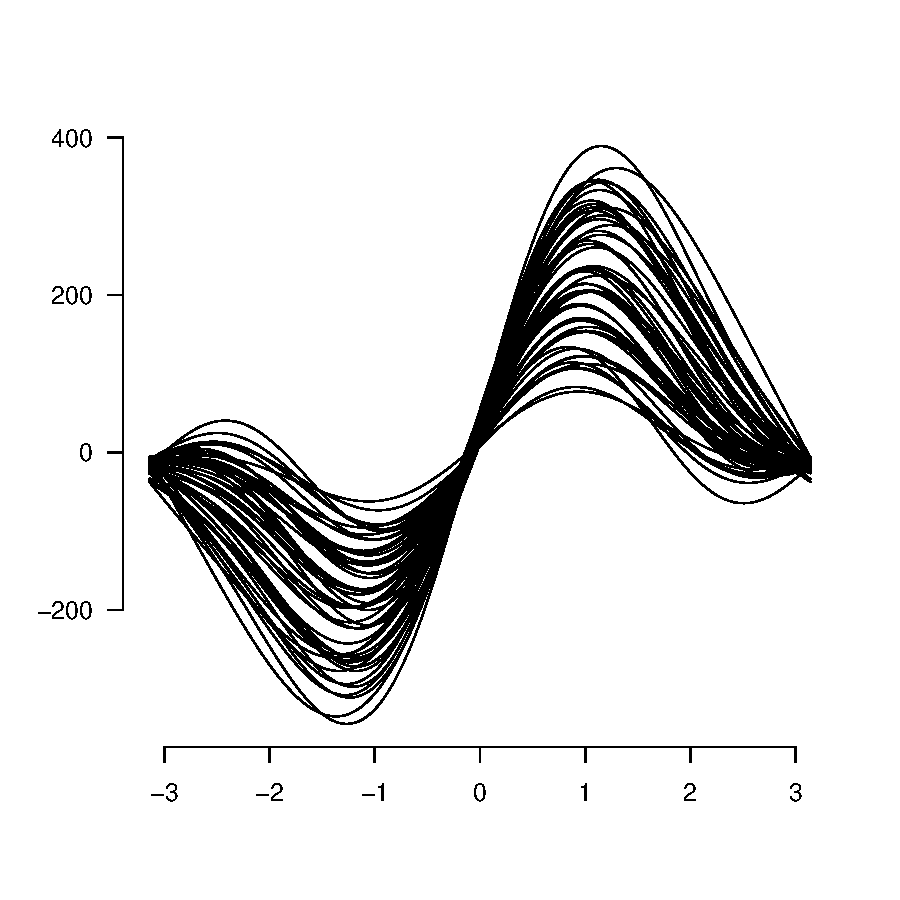
\includegraphics[width = 0.5\textwidth]{images/andrews}
\caption{Andrews Curves of US arrests data}
\end{center}
\end{figure}

You may like to consider at some stage (perhaps not today) how you could write an R function that plots Andrew's curves?   (there's a function in the \texttt{mvmmisc.R} file).

Try creating a matrix of data values from Fisher's Iris data, and a column of species names.   Then call up the andrews curves function:

\singlespacing
\begin{verbatim}
> iris.data <- iris[,-5]
> iris.species <- iris[,5]
> andrews.curves(iris.data, iris.species)
\end{verbatim}
\onehalfspacing


However, a simpler profile plots is available from the MASS library:

\singlespacing
\begin{verbatim}
> library(MASS)
> parcoord(USArrests)
\end{verbatim}
\onehalfspacing

The idea is that not only are the values of each individual variable represented, but also the patterns of different individuals can be seen.

If you now try looking at Fisher's Iris data (the [,-5] drops the species column which is a factor and cannot be plotted)

\singlespacing
\begin{verbatim}
> parcoord(iris[,-5])
\end{verbatim}
\onehalfspacing

You can also tell \texttt{parcoord()} to colour the profiles in according to the species.

\singlespacing
\begin{verbatim}
> parcoord(iris[,-5], col = as.numeric(iris[,5]))
\end{verbatim}
\onehalfspacing


\section{Animated exploration}

\begin{figure}
\begin{center}
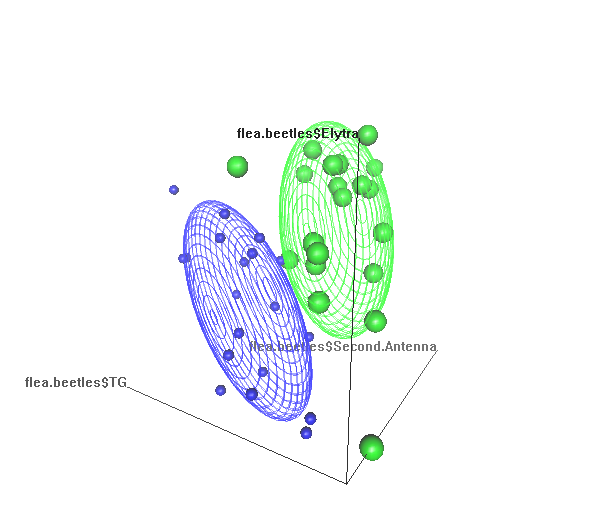
\includegraphics[width = 0.5\textwidth]{images/rgl}
\caption{rgl animated view of first three variables of flea beetle data}
\label{rgl}
\end{center}
\end{figure}

This shows an rgl with ellipsoids.


%\section{Dimension reduction}
%\label{dr}
%\section{Measures of distance}
%\label{distance}



%\section{Exercises}

%Hopefully the above examples, based on the USArrests data, give you some ideas as to how we start to visualise multivariate data.   We will consider more specialised methods (such as biplots and other projection methods) as the course progresses.   This week, you are strongly encouraged to consider how you could visualise the following datasets (all within R).

%\singlespacing
%\begin{itemize}
%\item attitude (survey of employees in different departments of a firm)
%\item longley (economic data)
%\item swiss (fertility and socio-economic data)
%\item USJudgeRatings (how lawyers rate judges in the US)
%\end{itemize}
%\onehalfspacing

You can use the help system to find more information on the datasets (e.g. type \texttt{> ?longley}).
%
%\fbox{Consider suitable methods for presenting these data.}

%%% Local Variables: ***
%%% mode:latex ***
%%% TeX-master: "../book.tex"  ***
%%% End: ***